\documentclass[10pt,a4paper]{book}

\usepackage{colordvi,epsfig,amsmath,xspace,fancyvrb,wrapfig}
\usepackage{fullpage}

\newcommand{\ie}{i.e.\@\xspace}
\newcommand{\R}{\mbox{$I\!\!R$}}
\newcommand{\E}{\mbox{$I\!\!E$}}
\newcommand{\Var}{\mathrm{Var}}

\begin{document}

\title{SML User Guide \\
Structure-Conveying Modelling Language reference}
\author{Marco Colombo\thanks{Email: {\tt M.Colombo@ed.ac.uk}}
\and Andreas Grothey\thanks{Email: {\tt A.Grothey@ed.ac.uk}}
\and Jonathan Hogg\thanks{Email: {\tt J.Hogg@ed.ac.uk}}
\and Kristian Woodsend\thanks{Email: {\tt K.J.Woodsend@sms.ed.ac.uk}}
\and Jacek Gondzio\thanks{Email: {\tt J.Gondzio@ed.ac.uk}} \\[3ex]
School of Mathematics, \\ University of Edinburgh, UK
}

\date{\today}

\maketitle

\section*{Foreward}
\label{sec:Intro}

Algebraic modelling languages are recognised as an important tool in the
formulation of mathematical programming problems. They facilitate the
construction of models through a language that resembles mathematical
notation, and offer convenient features such as automatic differentiation and
direct interfacing to solvers. Their use vastly reduces the need for tedious
and error-prone coding work. Examples of popular modelling languages
are AMPL \cite{mybib:AMPL}, GAMS \cite{mybib:GAMS}, AIMMS \cite{mybib:AIMMS}
and Xpress-Mosel \cite{mybib:Mosel}.

SML (Structured Modelling Language) attempts build on these traditional
approaches while encapsulating the {\bf structure} of the problem. As such
it encapsulates the AMPL syntax in an object orientated fashion.

It would be greatly appreciated if users would cite the following references
in work that uses SML:
\begin{itemize}
   \item {\it A Structure Conveying Parallelizable Modeling Language for Mathematical Programming}, Andreas Grothey, Jonathan Hogg, Kristian Woodsend, Marco Colombo and Jacek Gondzio, {\bf Springer Optimization and Its Applications Vol. 27: Parallel Scientific Computing and Optimization ed: R.Ciegis, D.Henty, B.K\r{a}gstr\"{o}m, and J.\v{Z}ilinska. 2009.}
\end{itemize}

%%%%%%%%%%%%%%%%%%%%%%%%%%%%%%%%%%%%%%%%%%%%%%%%%%%%%%%%%%%%%%%%%%%%%%%%%%%%
\chapter{Installation}
SML uses the standard GNU autotools install process. This can be summarised
by the following steps:
\begin{enumerate}
   \item ./configure --with-ampl=/path/to/amplsolver
   \item make
   \item make install
\end{enumerate}

In order to build correctly SML needs to know the location of the AMPL Solver
library. This is freely available to download from 
http://www.netlib.org/ampl/solvers/ and you need to supply the directory
containing the final libamplsolver.a to configure's --with-ampl= argument.
Further, SML {\it requires} AMPL to be installed to run. You can purchase a
copy of AMPL from one of the suppliers listed on the AMPL webpage at 
http://www.ampl.com/vendors.html and the shell command ampl should invoke it.

SML currently offers two solver interfaces:
\begin{description}
   \item{MPS} which will output the problem to an MPS file but will
      lose the strctural information in the process.
   \item{OOPS} which requires the OOPS and MeTiS libraries.
\end{description}

For information on the Object Orientated Parallel Solver (OOPS) please
contact Jacek Gondzio or see his webpage http://www.maths.ed.ac.uk/~gondzio/parallel/solver.html . The MeTiS graph partitioning software used by OOPS is
available from the Karypis lab at http://glaros.dtc.umn.edu/gkhome/views/metis .
 The locations of these packages can be passed to configure using the options
 --with-metis=/path/to/metis/base/dir and --with-oops=/path/to/oopshome .

 To surpress the compilation of the MPS interface use the option --with-mps=no .
 configure also offer several other options run ./configure --help for a
 more detailed summary.

%%%%%%%%%%%%%%%%%%%%%%%%%%%%%%%%%%%%%%%%%%%%%%%%%%%%%%%%%%%%%%%%%%%%%%%%%%%%
\chapter{Structured Problems}
\label{background}

A typical mathematical programming problem can be written in the form
\begin{equation}
\min_x f(x)\; \text{~s.t.~} Ax=b,\, x\ge 0
\end{equation}
If the matrix $A$ is structured then this can be exploited by modern solvers
to solve the problem faster.

This structure can take a number of forms, for example if the problem involves
a network then the node-arc inicidence matrix may be repeated multiple times
within the matrix $A$, or if the problem is stochastic in nature then the
scenario tree can be exploited.

Throught this guide we will consider two strucuted problems:
\begin{description}
   \item[MSND] Survivable Network Design
   \item[ALM] Asset and Liability Management
\end{description}
and these will be described in the following sections.

\section{Example Problem: Survivable Network Design}
A network is described by sets $\mathcal{V}$ of nodes and
$\mathcal{E}$ of (directed) arcs and a base capacity $C_j$
for every arc $j\in\mathcal{E}$. The basic multi-commodity network flow
(MCNF) problem considers the best way to move commodities
$k\in\mathcal{C}$ from their sources to their respective destinations, through
the arcs of the shared-capacity network. Each commodity is described as the
triplet $(s_k, t_k, d_k)$ consisting of start node $s_k$, terminal
node $t_k$ and amount to be shipped $d_k$. A feasible flow 
$x_k = (x_{k,j})_{j\in\mathcal{E}}$ for the $k$-th commodity can be
represented by the constraint
$$
A x_k = b_k, \quad x_k\ge 0,
$$
where $A\in\R^{|\mathcal{V}|\times|\mathcal{E}|}$ is the node--arc
incidence matrix, and $b_k = (b_{k,i})_{i\in\mathcal{V}}$ is the demand vector
for the $k$-th commodity, with the following conventions:\\
\parbox{8cm}{
$$
A_{i,j} = \left\{\begin{array}{rl}
 -1 \quad & \text{node $i$ is source of arc $j$},\\
  1 \quad & \text{node $i$ is target of arc $j$,}\\
  0 \quad & \text{otherwise},
\end{array}\right.
$$
}
\parbox{8cm}{
$$
b_{k,i} = \left\{\begin{array}{rl}
 -d_k \quad & \text{node $i$ is source of demand $k$},\\
  d_k \quad & \text{node $i$ is target of demand $k$},\\
  0 \quad & \text{otherwise}.
\end{array}\right.
$$
}\\
In multi-commodity survivable network design (MSND) the aim is to 
find the minimum installation cost of additional (spare) capacities
$S_j$ at price $c_j$, $j\in\mathcal{E}$, so that the given commodities
can still be routed through the network if any one arc or node should fail.
The MSND problem can be modelled by a series of multi-commodity network flow
problems, in each of which one of the original arcs or nodes is removed.
Note that the subproblems are not completely independent, as they
are linked by the common spare capacities $S_j$.

Let $A^{(a,l)}$, $l\in\mathcal{E}$, be the node--arc incidence matrix in
which the column corresponding to the $l$-th arc is set to zero. Then any
vector of flows $x_k^{(a,l)}\ge 0$ satisfying
\[
A^{(a,l)} x_k^{(a,l)} = b_k,\quad k \in\mathcal{C},\, l\in\mathcal{E},
\]
gives a feasible flow to route the $k$-th commodity through the
arc-reduced network. Similarly let $A^{(n,i)}$, $i\in\mathcal{V}$, be the node--arc incidence matrix in
which the row corresponding to the $i$-th nodes and the columns
corresponding to arcs incident to this node are set to zero. Then any
vector of flows $x_k^{(n,i)}\ge 0$ satisfying
\[
A^{(n,i)} x_k^{(n,i)} = b_k,\quad k \in\mathcal{C},\, i\in\mathcal{V},
\]
gives a feasible flow to route the $k$-th commodity through the
node-reduced network. 
As the network is capacity-limited, however,
each arc $j\in\mathcal{E}$ can carry at most
$C_j + S_j$ units of flow. 
The complete formulation of the MSND problem is as follows:
\begin{equation}
\begin{array}{rll}
\min & \displaystyle \sum_{j \in \mathcal{E}} c_j S_j\\
\text{s.t.} & A^{(a,l)} x_k^{(a,l)} = b_k
                  & \;\forall k\in\mathcal{C},l\in\mathcal{E}\\
            & A^{(n,i)} x_k^{(n,i)} = b_k
                  & \;\forall k\in\mathcal{C},i\in\mathcal{V}\\
            & \displaystyle \sum_{k\in\mathcal{C}} x_{k,j}^{(a,l)} \le C_j + S_j 
                   & \;\forall j\in\mathcal{E}, l\in \mathcal{E}\\
            & \displaystyle \sum_{k\in\mathcal{C}} x_{k,j}^{(n,i)} \le C_j + S_j 
                   & \;\forall j\in\mathcal{E}, i\in \mathcal{V}\\
            & x, s \ge 0
\end{array}\label{MSND}
\end{equation}

\begin{figure}[ht]
\begin{center}
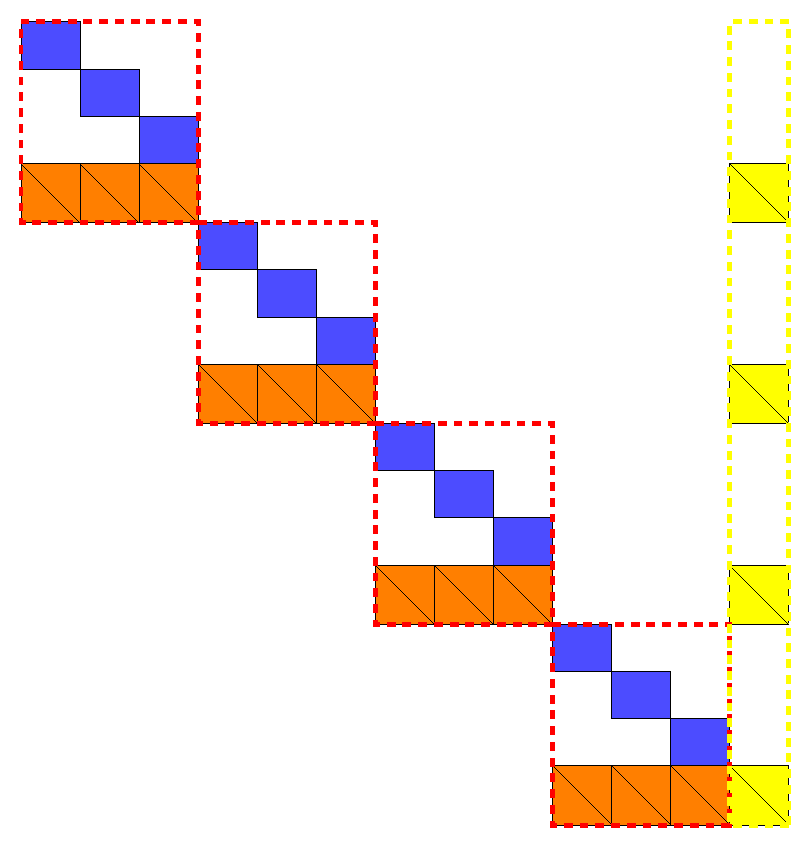
\epsfig{file=fig/MSND_struct,width=7cm}
\end{center}
\caption{Structure of the constraint matrix for the MSND problem.}
\label{MSND_struct}

\end{figure}
%

The constraint matrix of this problem has the form shown in Figure~\ref{MSND_struct}.
The basic building blocks are the node--arc incidence matrices (shown in dark grey).
These blocks are repeated for every commodity that
needs to be shipped, and they are linked by a series of common rows
(shown in medium grey)
that represent the global capacity constraints to build a MCNF
problem. Each MCNF block (framed by dashed lines) is repeated for every (missing) arc
and node. The common capacity variables (light grey blocks) act as linking
columns. 
While the nested structure of the problem is obvious is
Figure~\ref{MSND_struct}, it cannot be easily appreciated from the mathematical
formulation (\ref{MSND}).

%
%
\subsection{Standard modelling language formulation}

Problem \eqref{MSND} can be represented in an algebraic
modelling language as shown in Figure~\ref{AMPLMSND}, where we adopt a
syntax that is very close to AMPL, slightly modified to compress the example
and aid readability; models in other languages will look much the same.
%
\begin{Verbatim}[frame=single,framerule=0.2pt,framesep=5pt,commandchars=\\\{\}]
\Red{set} NODES, ARCS, COMM;
\Red{param} cost\{ARCS\}, basecap\{ARCS\};
\Red{param} arc_source\{ARCS\}, arc_target\{ARCS\};
\Red{param} comm_source\{COMM\}, comm_target\{COMM\}, comm_demand\{COMM\};
\Red{param} b\{k in COMM, i in NODES\} := 
  if  (comm_source[k]==i) then comm_demand[k] else 
    if (comm_target[k]==i) then -comm_demand[k] else 0;

\textit{\Gray{# first index is missing arc/node, then commodity, then arc of flow}}
\Red{var} Flow\{ARCS union NODES, COMM, ARCS\} >= 0;
\Red{var} sparecap\{ARCS\} >= 0;
 
\textit{\Gray{# flow into node - flow out of node equals demand}}
\Red{subject to} FlowBalanceMissingArcs\{a in ARCS, k in COMM, i in NODES\}:
  sum\{j in ARCS:j~=a, arc_target[j]==i\} Flow[a,k,j]  
   - sum\{j in ARCS:j~=a, arc_source[j]==i\} Flow[a,k,j] = b[k,i]; 

\Red{subject to} FlowBalanceMissingNodes\{n in NODES, k in COMM, i in NODES diff \{n\}\}:
  sum\{j in ARCS:arc_target[j]==i, arc_source[j]~=n\} Flow[n,k,j]  
   - sum\{j in ARCS:arc_source[j]==i, arc_target[j]~=n\} Flow[n,k,j] = b[k,i]; 

\Red{subject to} CapacityMissingArcs\{a in ARCS union NODES, j in ARCS\}:
   sum\{k in COMM\} Flow[a,k,j] <= basecap[j] + sparecap[j];

\Red{minimize} obj: sum\{j in ARCS\} sparecap[j]*cost[j];
\end{Verbatim}

\section{Example Problem: Asset and Liability Management}

As an example of a stochastic programming problem we use an asset and
liability management problem.
The problem is concerned with investing an initial cash amount $b$ into
a given set of assets $\mathcal{A}$ over $T$ time periods in such a way
that, at every time stage $0 < t \le T$, a liability payment $l_t$ 
can be covered.
Each asset has value $v_j$, $j\in\mathcal{A}$.
The composition of the portfolio can be changed throughout the investment
horizon, incurring (proportional) transaction costs $c$,
$x_{i,j}^h$ is the amount of asset $j$ held at node $i$,
$x_{i,j}^b$ and $x_{i,j}^s$ are the amounts bought and sold.
These satisfy the inventory and cash balance equations at every node.
The random parameters are the asset returns $r_{i,j}$ that hold
for asset $j$ at node $i$.
The evolution of uncertainties can be described by an event tree:
For a node $i$, $\pi(i)$ is its parent in the tree,
$p_i$ is the probability of reaching it, 
and $\tau(i)$ represents its stage.
With $\mathcal{L}_T$ we denote the set of final-stage nodes.
%
The objective maximises a linear combination of the expectation of the final
portfolio value (denoted by $\mu$) and its variance, with risk-aversion
parameter $\lambda$:
\[
 \max \{\E(wealth) - \lambda\Var(wealth)\} = 
 \max \{\E\left(wealth - \lambda \left[wealth^2 - \E(wealth)^2\right]\right)\}.
\]


The complete model is the following:
\begin{eqnarray}
\max_{x,\,\mu\ge 0}&& \mu - \rho[\sum_{i\in\mathcal{L}_T}
p_i [(1-c)\sum_{j\in\mathcal{A}} v_j x_{i,j}^h]^2 - \mu^2]\notag\\
\text{~s.t.~}&&
\begin{array}[t]{rcll}
x_{i,j}^h &=& (1+r_{i,j})x_{\pi(i),j}^h +  x_{i,j}^b - x_{i,j}^s,&\forall i\ne 0, j\in\mathcal{A}\\
\sum_{j\in\mathcal{A}} (1-c) v_j x_{i,j}^s &=& l_{\tau(i)} + \sum_{j\in\mathcal{A}} (1+c) v_j x_{i,j}^b, &\forall i\ne 0\\ 
\sum_{j\in\mathcal{A}} (1+c) v_j x_{0,j}^b &=& b\\
 (1-c) \sum_{i\in \mathcal{L}_T} p_i\sum_{j\in\mathcal{A}} v_j x_{i,j}^h &=& \mu
\end{array}
\label{alm}
\end{eqnarray}

\section{Identifying structure}

So how do we identify strcuture? Generally if you are building you model out
of repeated components you can easily obtain strucutre - it may be that this
strucutre would be indexed over in the tradional Algerbraic Modelling Language
representation - for example the indexing over {\tt ARCS} and {\tt NODES} in
the MSND example, and the indexing over the scenario tree in the stochastic
ALM example.

If this indexing is pulled out into a series of related blocks then the
problem becomes similar. In the next example we consider the structured
representation of the MSND model.

\subsection{MSND Example}
Using the {\tt block} keyword, the previous MSND model can be rewritten as:

\begin{Verbatim}[frame=single,framerule=0.2pt,framesep=5pt,commandchars=\\\{\}]
\Red{set} NODES, ARCS, COMM;
\Red{param} cost\{ARCS\}, basecap\{ARCS\};
\Red{param} arc_source\{ARCS\}, arc_target\{ARCS\};
\Red{param} comm_source\{COMM\}, comm_target\{COMM\}, comm_demand\{COMM\};
\Red{param} b\{k in COMM, i in NODES\} := 
  if  (comm_source[k]==i) then comm_demand[k] else 
    if (comm_target[k]==i) then -comm_demand[k] else 0;

\Red{var} sparecap\{ARCS\} >= 0;

\Red{block} MCNFArcs\{a in ARCS\}: \{
  \Red{set} ARCSDIFF = ARCS diff \{a\};  \textit{\Gray{# local ARCS still present}}

  \Red{block} Net\{k in COMM\}: \{
    \Red{var} Flow\{ARCSDIFF\} >= 0;
    \textit{\Gray{# flow into node - flow out of node equals demand}} 
    \Red{subject to} FlowBalance\{i in NODES\}:
      sum\{j in ARCSDIFF:arc_target[j]==i\} Flow[j]  
      - sum\{j in ARCSDIFF:arc_source[j]==i\} Flow[j] = b[k,i];  
  \}

  \Red{subject to} Capacity\{j in ARCSDIFF\}:
     sum\{k in COMM\} Net[k].Flow[j] <= basecap[j] + sparecap[j];
\}

\Red{block} MCNFNodes\{n in Nodes\}: \{
  \Red{set} NODESDIFF = NODES diff \{n\};\textit{\Gray{ # local NODES still present}}
  \Red{set} ARCSDIFF = \{i in ARCS: arc_source[i]~=n, arc_target[i]~=n\};

  \Red{block} Net\{k in COMM\}: \{
    \Red{var} Flow\{ARCS\} >= 0;
    \textit{\Gray{# flow into node - flow out of node equals demand}} 
    \Red{subject to} FlowBalance\{i in NODESDIFF\}:
      sum\{j in ARCSDIFF:arc_target[j]==i\} Flow[j]  
      - sum\{j in ARCSDIFF:arc_source[j]==i\} Flow[j] = b[k,i];  
  \}

  \Red{subject to} Capacity\{j in ARCSDIFF\}:
     sum\{k in COMM\} Net[k].Flow[j] <= basecap[j] + sparecap[j];
\}

\Red{minimize} costToInstall: sum\{j in ARCS\} sparecap[j]*cost[j];
\end{Verbatim}

\section{Stochastic Structure}

As stochastic programming is a common source of such strucutred problems, and
the special conventions used to represent stochastic entities, SML includes
some special conventions for handling stochastic problems. Our next example
shows these in action.

\subsection{ALM Example}

\begin{Verbatim}[frame=single,framerule=0.2pt,framesep=5pt,commandchars=\\\{\}]
\Red{param} Budget, T, Tc, Rho;
\Red{set} ASSETS, NODES, STAGES := 0..T;
\Red{param} PARENT\{NODES\} symbolic, PROBS\{NODES\};
\Red{param} Value\{ASSETS\};
\Red{var} mu;

\Red{block} alm stochastic using (NODES, PARENT, PROBS, STAGES):\{

  \Red{var} xh\{ASSETS\} >= 0, xb\{ASSETS\} >= 0, xs\{ASSETS\} >= 0;
  \Red{param} Ret\{ASSETS\};
  \Red{param} Liability deterministic;

  stage \{0\}: \{
    \Red{subject to} StartBudget:
      (1+Tc)*sum\{j in ASSETS\} xb[j]*Value[j] <= Budget;
  \}

  stage \{1..T\}: \{
    \Red{subject to} Inventory\{j in ASSETS\}:
      xh[j] = (1+Ret[j]) * ancestor(1).xh(j) + xb[j] - xs[j];
    \Red{subject to} CashBalance:
      (1-Tc) * sum\{j in ASSETS\} Value[j]*xs[j] = 
	 Liability + (1+tc)*sum\{j in ASSETS\} Value[j]*xb[j];
  \}

  stage \{T\}: \{
    \Red{var} wealth := (1-tc) * sum\{j in ASSETS\} Value[j]*xh[j];
    \Red{subject to} ExpPortfolioValue:
      Exp(wealth) = mu;
    \Red{maximize} objFunc: mu - Rho * ((wealth*wealth) - mu*mu )
  \}
\}
\end{Verbatim}

%%%%%%%%%%%%%%%%%%%%%%%%%%%%%%%%%%%%%%%%%%%%%%%%%%%%%%%%%%%%%%%%%%%%%%%%%%%%
\chapter{SML Keywords}
In order to facilitate Structured Modelling we have introduced several new
keywords and structures into the AMPL langauge.

\section{Blocks}
A block is defined as follows:

\begin{Verbatim}[commandchars=\\\{\}]
   block \textit{nameofblock}\{[j in] \textit{set_expr}\}: \{
     [statements]
   \}
\end{Verbatim}
Between the curly braces {\tt \{\}} , any number of {\tt set, param,
subject to, var, minimize} or indeed further {\tt block} definitions can be
placed. The interpretation is that all declarations placed inside the block
environment are implicitly repeated over the indexing expression used for the
{\tt block} command. Clearly, the nesting of such {\tt block}s creates a tree
structure of blocks.

A block introduces the notion of scope, similar to that found in the programming
language C. Within a block all references to objects visible to the containing
context are visible {\it unless} there is an object with the same name defined
within the block.

\section{Stochastic Blocks and Variables}
A stochastic program is declared in SML via the {\tt stochastic} modifier
to the {\tt block} command:
\begin{Verbatim}[commandchars=\\\{\}]
  block \textit{nameofblock} stochastic using(NODES, PROB, PARENT, STAGES): \{
     stochastic statements
  \}
\end{Verbatim}
where the expressions {\tt NODES, PROB, PARENT} and {\tt STAGES} conform to
the following relations:
\begin{verbatim}
  set NODES; 
  param PROB{NODES};
  param PARENT{NODES} symbolic, within (NODES union {none});
  set STAGES ordered;  
\end{verbatim}
The {\tt stochastic statements} include both normal AMPL and {\tt block}
statements, but may also include the special {\tt stage} statement:
\begin{verbatim}
  stage set_expr: {
    ...
  }
\end{verbatim}
that declares variables and constraints which apply only to the specific stages
in the supplied set expression.

The scenario tree is defined by the set of {\tt NODES} and their {\tt PARENT}
relationship. The probability associated with a node is the conditional
probability of reaching that node given that its parent is reached. The
set expression STAGES is used only to provide labels for the stages should
they be required.

Entites defined within the stochastic block are either {\it stochastic} and
are repeated for nodes in their {\it stageset}, or are {\it deterministic} and
are repeated only once for each stage. By default entities are stochastic
and their stageset is the full set STAGES. Entities within a {\tt stage} block
are by default stochastic with their stageset determined by the {\tt stage} set
expression.

The nature of an entity may be changed from the default through the use of the
special attributes {\tt deterministic} and {\tt stage set\_expr} in their
declaration.

Relations between different stages can be expressed by using the 
{\tt ancestor(i)} function that allows to reference the $i$-th ancestor
stage. Variables of the ancestor can be referenced using the normal SML syntax,
{\tt ancestor(i).x}.

Expectations may also be handled through a special new syntax. Within a
stochastic block the expresion {\tt Exp(expr)} is equivilant to the expression
{\tt sum\{nd in NODES: nd in \textit{currentstage}\} PROBS[nd] * expr[nd]}.

%%%%%%%%%%%%%%%%%%%%%%%%%%%%%%%%%%%%%%%%%%%%%%%%%%%%%%%%%%%%%%%%%%%%%%%%%%%%
\chapter{Advanced Topics}

\section{Solver Interface}
\label{interface}

If you wish to hook a solver other than OOPS to SML then you will need to use
the interface described in this section. We first describe the data
representation used by the interface before describing the available function
calls. The implementor is advised to browse the source code for the MPS
interface for an example implementation.

\subsection{Data strcuture}
Internally  SML describes a problem as a nested bordered block diagonal form.
The data structure used to represent this assumes the following:
\begin{enumerate}
   \item A block has a zero or more constraints of variables with an associated
      Jacobian matrix, labelled A in Figure~XXX.
   \item Further, associated variables may contribute to the objective function.
   \item A block has zero or more additional blocks nested within it, these are
      represented by a list of pointers to the contained blocks.
   \item A contained block has a similar internal structure, labelled B, that
      has no bearing on the constraints of varibles associated with this block.
   \item The constrained block may contain constraints on the variables
      associated with this block, with a jacobian labelled C.
   \item This block may place constraints upon variables associated with
      the contained block, ielding the jacobian labelled D.
   \item Any or all of the jacobians A, B, C or D may be identically zero.
\end{enumerate}

Clearly the list of pointers to contained blocks yields a tree strucutre which
we refer to as the Expanded Model Tree.  This representation of the structured
model is natural for a hierarchical linear algebra solver such as OOPS, but
should also provide sufficient access for other designs of structure exploiting
solver such as those which use decompopsition approaches.

\subsection{Basic Use}

The model currently used by SML is that it is called by the solver and passed
the names of the model and data files, it will then return a pointer to an
Expanded Model Tree represented by a {\tt ModelInterface} object which the
solver is then free to query. Finally the solver should {\tt delete} the
{\tt ModelInterface} object to free the memory.

We recommend that most solvers parse the tree in either one or two passes. The
inital parse may extract information on the dimension and relative density of
the tree, setting up data structures are required, while the second pass will
determine the actual numeric values.

\subsection{API}

\subsubsection{Aquiring the ModelInterface object}
The solver should use the include statement
\begin{verbatim}
#include "sml.h"
\end{verbatim}
which will provide access to all relevant definitions. The solver should then
call the function:

\begin{verbatim}
ModelInterface* sml_generate(const std::string modelfilename, const std::string datafilename, const bool debug);
\end{verbatim}

to retrieve a {\tt ModelInterface} object which can then be queried. If the
argument {\tt debug} is {\tt true} then additional debugging information will
be generated.

\subsubsection{Transversing the Tree}
The {\tt ModelInterface} object returned after parsing the model and data files
offers two iterators for movign through the tree, and further allows direct
access to the list of children.

The {\tt ModelInterface::ancestor\_iterator} allows the iteration up through
the tree to the root. The function {\tt ModelInterface::abegin()} returns an
iterator which points to the parent of the node it is called on. The function
{\tt ModelInterface::aend()} return an iterator which represents the top of the
tree, above the root.

The {\tt ModelInterface::child\_iterator} allows the iteration over all children
of a node in a depth-first order, with the node itself being last. The function
{\tt ModelInterface::cbegin()} returns an iterator pointing to the left-most
leaf in the subtree routed at the calling node. The function 
{\tt ModelInterface::cend()} returns an iterator representing the end of the
child iteration sequence.

The comonent {\tt std::vector<ModelInterface*> ModelInterface::children} allows
the solver writer to use their own iteration scheme if the above are not
sufficient.

We note that (non-)equivilance of pointers is not a sufficient condition to
differentiate nodes, and the function {\tt std::string ModelInterface::getName()} should be used instead.

\subsubsection{Accessing the Data}
Each block essentially allows the query of all data in its row block. The
following functions are available:
\begin{tabular}{ll}
{\tt int getNLocalVars()} & 
   Number of variables local to block \\
{\tt const std::list<std::string>\& getLocalVarNames()} &
   List of variable names local to block \\
{\tt int getNLocalCons()} & 
   Number of constraints local to block \\
{\tt const std::list<std::string>\& getLocalConNames()} &
   List of constraint names local to block \\
\multicolumn{2}{l}{\tt int getNzJacobianOfIntersection(ModelInterface *emcol)}\\
\multicolumn{2}{r}{Number of non-zeros in submatrix in block column {\tt emcol}
   and this block row} \\
\multicolumn{2}{l}{\tt void getJacobianOfIntersection(ModelInterface *emcol,
      *colbeg, *collen, *rownbs, *el)} \\
\multicolumn{2}{r}{Entries of submatrix in block column {\tt emcol} and this
   block row, in CSC format (see below)} \\
{\tt void getRowLowBounds(double *elts)} &
   Constraint lower bounds for block. \\
{\tt void getRowUpBounds(double *elts)} &
   Constraint upper bounds for block. \\
{\tt void getColLowBounds(double *elts)} &
   Variable lower bounds for block. \\
{\tt void getColUpBounds(double *elts)} &
   Variable upper bounds for block. \\
{\tt void getObjGradient(double *elts)} &
   Objective coefficients for block.
\end{tabular}

The Compressed Sparse Column (CSC) format used by 
{\tt getJacobianOfIntersection()} describes for each column only the non-zero
entries within it, and for each entry gives a row number and value pair. On
entry the parameters should point to areas of memory corresponding to the
following arrays: {\tt int colbeg[n+1], int collen[n], int rownbs[nz],
double el[nz]}, where {\tt n} is the number of variables in this model, and
{\tt nz} is the number returned by the corresponding call to
{\tt getNzJacobianOfIntersection()}.

On return {\tt colbeg[i]} is a pointer to the begining of column {\tt i}
within the arrays {\tt rownbs[]} and {\tt el[]}, {\tt collen[i]} is the number
of entries in that column --- which may be zero. The values {\tt rownbs[j]} and
{\tt el[j]} represent a row number-value pair.

\section{Implementation} \label{implementation}

SML is implemented in the object-oriented C++ language as a
pre- and post-processor to AMPL.  
The SML model file
is parsed to extract the prototype model-tree, the list of entities
associated with each prototype-tree node and the dependency graph of
the entities. 
The goal of the pre-processing stage is to create, for each node in the
prototype model-tree, a stand-alone AMPL model file that describes the
local model for this block of the problem. 
The file includes definitions for all the
entities belonging to the prototype-tree node and all their
dependencies: references to entities are changed to a
global naming and indexing scheme, that easily generated from the
SML model file by generic text substitutions.  
Figure~\ref{AMPLsubmodMCNF} shows these AMPL submodel files for the MSND problem formulation. 

% Variable and constraint definitions in the submodel files are very similar to the ones in the original unstructured AMPL model. 
% By means of the SML description we have managed to separate the AMPL model into the appropriate submodels for every node of the prototype model tree.
The AMPL model is separated into the appropriate submodels for every node
of the prototype tree by changing the indexing sets.
Each block definition is replaced
by declaring an indexing set (named {\tt *\_SUB}) for the
indexing expression of the sub-block, and this is prepended to the
indexing expressions of every entity declared in the sub-block. By
temporarily defining the set {\tt ARCS\_SUB} to a suitable subset of {\tt ARCS} 
(leveraging AMPL's scripting commands), the
model for any node on the expanded tree can be generated from the
corresponding submodel {\tt *.mod} file shown in Figure~\ref{AMPLsubmodMCNF}.


\begin{figure}
{\small
\begin{Verbatim}[frame=single,framerule=0.2pt,framesep=5pt,commandchars=\\\{\}]
%------------------------------- root.mod --------------------------------
\Red{set} ARCS;
\Red{param} cost\{ARCS\};

\Red{var} sparecap\{ARCS\} >= 0;

\Red{minimize} obj: sum\{j in ARCS\} sparecap[j]*cost[j];
\end{Verbatim}
\begin{Verbatim}[frame=single,framerule=0.2pt,framesep=5pt,commandchars=\\\{\}]
% -------------------------- root_MCNFArcs.mod ----------------------------
\Red{set} ARCS, COMM;
\Red{param} basecap\{ARCS\};

\Red{var} sparecap\{ARCS\} >= 0;

\Red{set} ARCS_SUB within ARCS;
\Red{set} ARCSDIFF\{a in ARCS_SUB\} = ARCS diff \{a\};  \textit{\Gray{# local ARCS still present}}

\Red{var} MCNFArcs_Net_Flow\{a in ARCS_SUB, ARCSDIFF[a], k in COMM\} >= 0;
\Red{subject to} Capacity\{a in ARCS_SUB, j in ARCSDIFF[a]\}:
     sum\{k in COMM\} MCNFArcs_Net_Flow[a,k,j] <= basecap[j] + sparecap[j];
\end{Verbatim}
\begin{Verbatim}[frame=single,framerule=0.2pt,framesep=5pt,commandchars=\\\{\}]
% -------------------------- root_MCNFArcs_Net.mod ----------------------------
\Red{set} NODES, ARCS, COMM;
\Red{param} arc_source\{ARCS\}, arc_target\{ARCS\};
\Red{param} comm_source\{COMM\}, comm_target\{COMM\}, comm_demand\{COMM\};
\Red{param} b\{k in COMM, i in NODES\} := 
  if  (comm_source[k]==i) then comm_demand[k] else 
    if (comm_target[k]==i) then -comm_demand[k] else 0;

\Red{set} ARCS_SUB within ARCS;
\Red{set} ARCSDIFF\{a in ARCS\} = ARCS diff \{a\};  \textit{\Gray{# local ARCS still present}}

\Red{set} COMM_SUB within COMM;
\Red{var} MCNFArcs_Net_Flow\{a in ARCS_SUB, k in COMM_SUB, ARCSDIFF[a]\} >= 0;
\textit{\Gray{# flow into node - flow out of node equals demand}} 
\Red{subject to} MCNFArcs_Net_FlowBalance\{a in ARCS_SUB, k in COMM_SUB, i in NODES\}:
      sum\{j in ARCSDIFF[a]:arc_target[j]==i\} MCNFArcs_Net_Flow[a,k,j]  
      - sum\{j in ARCSDIFF[a]:arc_source[j]==i\} MCNFArcs_Net_Flow[a,k,j] = b[k,i];  
  \}
\}
\end{Verbatim}
\caption{Generated AMPL model files for the root MSND model and MCNF submodels}
\label{AMPLsubmodMCNF}
}
\end{figure}
%
This process of model expansion based on indexing sets results
in a {\tt *.nl} file for every node of the expanded model
tree; each file carries all the information about this node needed by a
solver. The underlying submodel is the same for all expanded-tree
nodes that correspond to the same prototype-tree node. However
they are produced with different data instances: namely different
choices of elements from the {\tt block}'s indexing sets.

The nodes of the prototype and the expanded tree are internally
represented as C++ objects that carry pointers to their children. 
Therefore, the prototype and expanded trees are themselves trees of C++ objects.
The {\tt ExpandedTreeNode} class provides information on the dimension
of the node (number of local constraints and variables) and a list of
its children; further, it provides methods to evaluate the Jacobian of
its local constraints with respect to the local variables of a second
{\tt ExpandedTreeNode} object. Information on the number of sparse
elements of this Jacobian block can be obtained prior to requesting
the complete sparse matrix description to enable the allocation of
sufficient memory. As argued above, these methods should satisfy
the needs of all different conceivable structure-exploiting solvers. A
full discussion of the {\tt ExpandedTreeNode} class can be found in
the SML documentation.

\bibliographystyle{siam}
\bibliography{userguide}

%
% End Document
%
\end{document}
